\section{Database overview}
\label{sec:database-overview}

To be able to use the data available at \whoscored\ for training an \gls{ann}, it should be stored on a computer data storage device in some way. As there are vast amounts of available data, and the data is highly connected, a good option is to store the data in a relational database. Relational databases are designed with relational models in mind, and is therefore a natural choice of storage. 

This section describes the database used for storing the data used in this report. The database is set up using MySQL version 5.7.


\subsection{Central data}

\cref{fig:database-central} shows the five most central database tables.

A \textit{region} is either a nation, continent, or \textit{International}. International covers tournaments spanning several continents, such as the FIFA World Cup. Continents cover tournaments spanning several countries within the same continent, such as the UEFA European Championship. Nations cover national tournaments, such as the English Premier League. Nations are also used for tracking the nationality of club teams and players.

A \textit{league} is a tournament, either a league or a knockout tournament. A tournament spans over several \textit{seasons}, given by the year the season starts. This makes it possible to differentiate two seasons from each other, such as the 2015-2016 and 2016-2017 seasons of the English Premier League.

A \textit{team} is either a club or national team. Teams are not directly connected to any leagues, as teams can be promoted or relegated.

A \textit{player} is a former or present football player. Players are not directly connected to any teams, as players may change team.

\begin{figure}
    \centering
    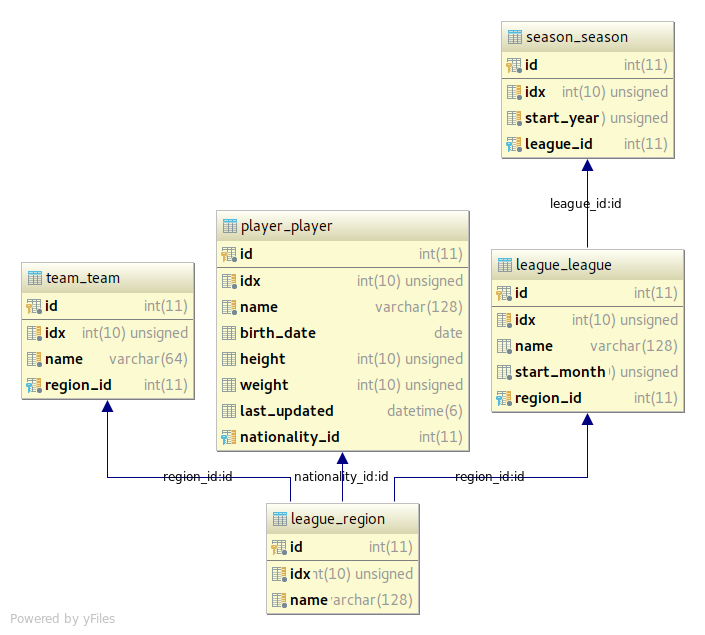
\includegraphics[width=0.9\textwidth]{database/central.png}
    \caption{Most central database tables.}
    \label{fig:database-central}
\end{figure}


\subsection{Matches}
\label{subsec:database-overview-matches}

\cref{fig:database-matches} shows the database tables containing information concerning matches.

A \textit{match} is a single match between two teams, the \textit{home team} and the \textit{away team}. Matches are played at a specific \textit{venue}, and is conducted by a specific \textit{referee}. All matches are part of a \textit{season}. Matches can be \textit{sparse}, meaning that they are covered by a minimum or intermediate level of details. Complete matches are marked with the Boolean attribute \textit{complete}. Matches that are postponed are marked with the \textit{postponed} attribute. For speeding up data fetching, two attributes, \textit{last\_matches\_fetched} and \textit{previous\_matches\_fetched}, marks whether the \textit{last matches} for the two teams, and the \textit{previous matches} between the teams have been fetched.

A \textit{previous meetings} instance lists the previous meetings between the two competing teams of a match. Previous meetings instances list a summary of the number of victories, goals scored, and cards issued for the two teams. For each match, there are three sets of previous meetings: one for the most recent matches, one for the most recent matches played at the home team venue, and one for the most recent matches played at the away team venue. These three sets are stored in the \textit{head to head} table.

It is possible to store a set of \textit{match odds} for a match. A match odds instance lists the odds for the three match outcomes (home victory, draw, or away victory) offered by a given \textit{bookmaker}.

\begin{figure}
    \centering
    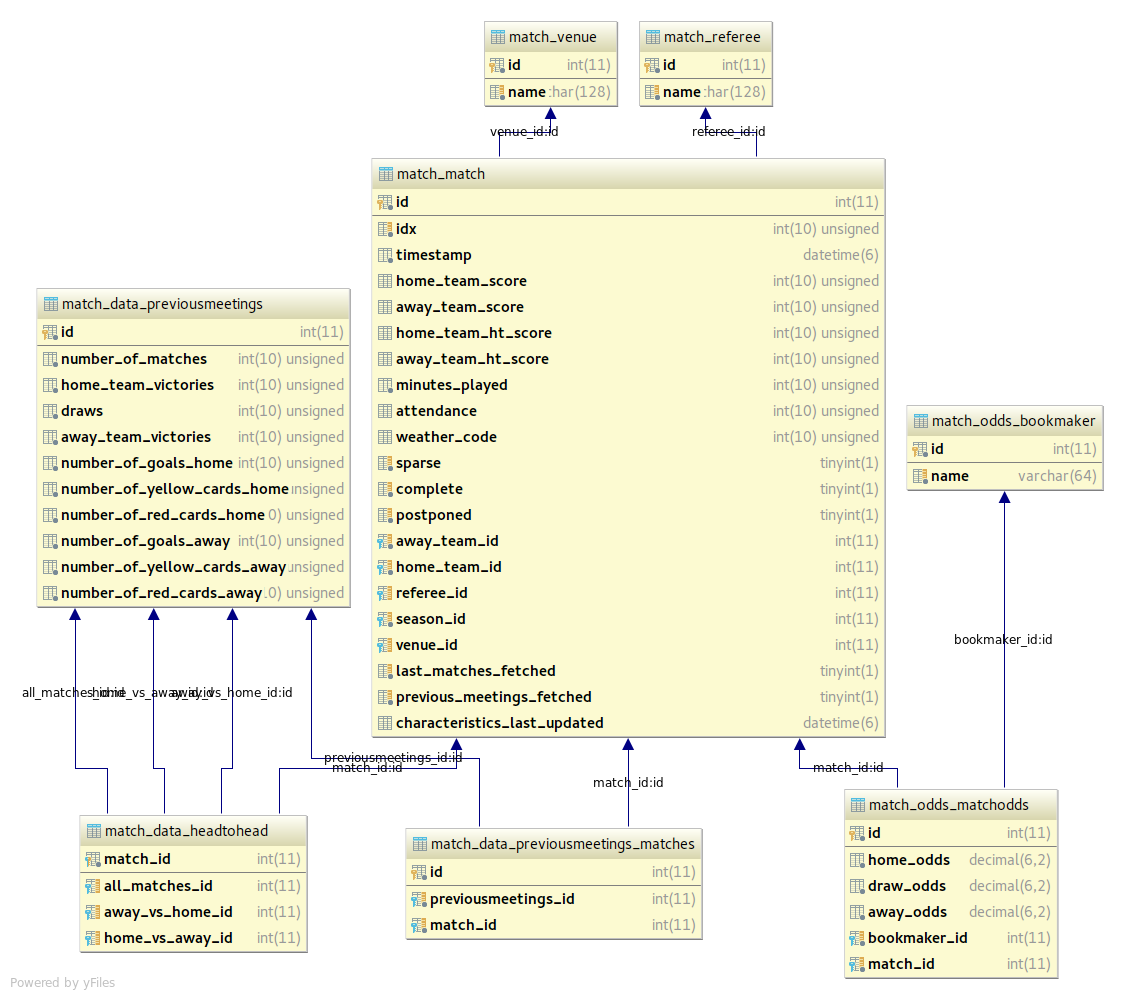
\includegraphics[width=0.9\textwidth]{database/match.png}
    \caption{Database tables containing match related information.}
    \label{fig:database-matches}
\end{figure}


\subsection{Team stats}
\label{subsec:database-overview-team-stats}

\cref{fig:database-team-stats} shows the database tables containing information concerning team stats.

A \textit{team stats} instance contains information concerning a team's participation in a match. For each match, there are two team stats, one for the home team, and one for the away team. A fully detailed team stats instance contains sets of \textit{ratings} and \textit{statistics}, developed over time, in addition to a final rating. Team ratings are sampled almost every minute and stored in the ratings set. The statistics contains a set for every metric in \cref{tab:whoscored-player-metrics}.

Each team stats instance has a set of associated \textit{team characteristics}. Characteristics are given by a type (offensive or defensive) and a name. A characteristic is either a strength, a weakness, or a style. Strengths and weaknesses have associated levels, ranging from 15 (very weak) to 55 (very strong).

\begin{figure}
    \centering
    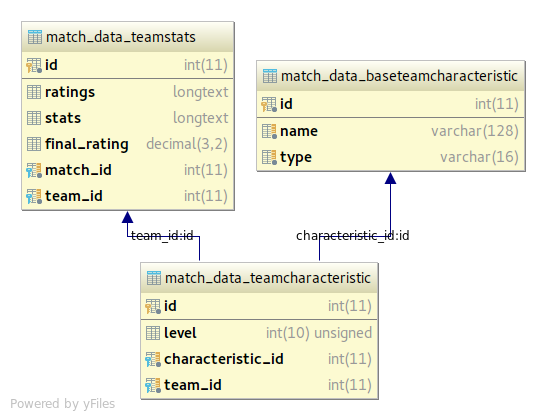
\includegraphics[width=0.9\textwidth]{database/team-stats.png}
    \caption{Database tables containing team stats related information.}
    \label{fig:database-team-stats}
\end{figure}


\subsection{Player stats}

\cref{fig:database-player-stats} shows the database tables containing information concerning player stats.

A \textit{player stats} instance contains information concerning a player's participation in a match. For each match, there are at least 22 player stats, one for each player. For matches with intermediate or full level of details, substitutes are also included. Player stats instances are marked with \textit{minute started} and \textit{minute ended}, marking what parts of the game the player participated in. A fully detailed player stats instance contains \textit{ratings} and \textit{statistics}, similar to those for team stats. In addition, player stats instances contain the final count for every metric in \cref{tab:whoscored-player-metrics}. Player stats are marked with two Boolean values, \textit{is\_first\_eleven} and \textit{is\_man\_of\_the\_match}, signaling whether the player started the match or was rated man of the match, respectively. A player stats instance is also associated with a \textit{player position}, such as \textit{goal keeper}, \textit{left back}, etc.

\textit{Player characteristics}, are not associated with a specific match, but rather with the player object itself.

\begin{figure}
    \centering
    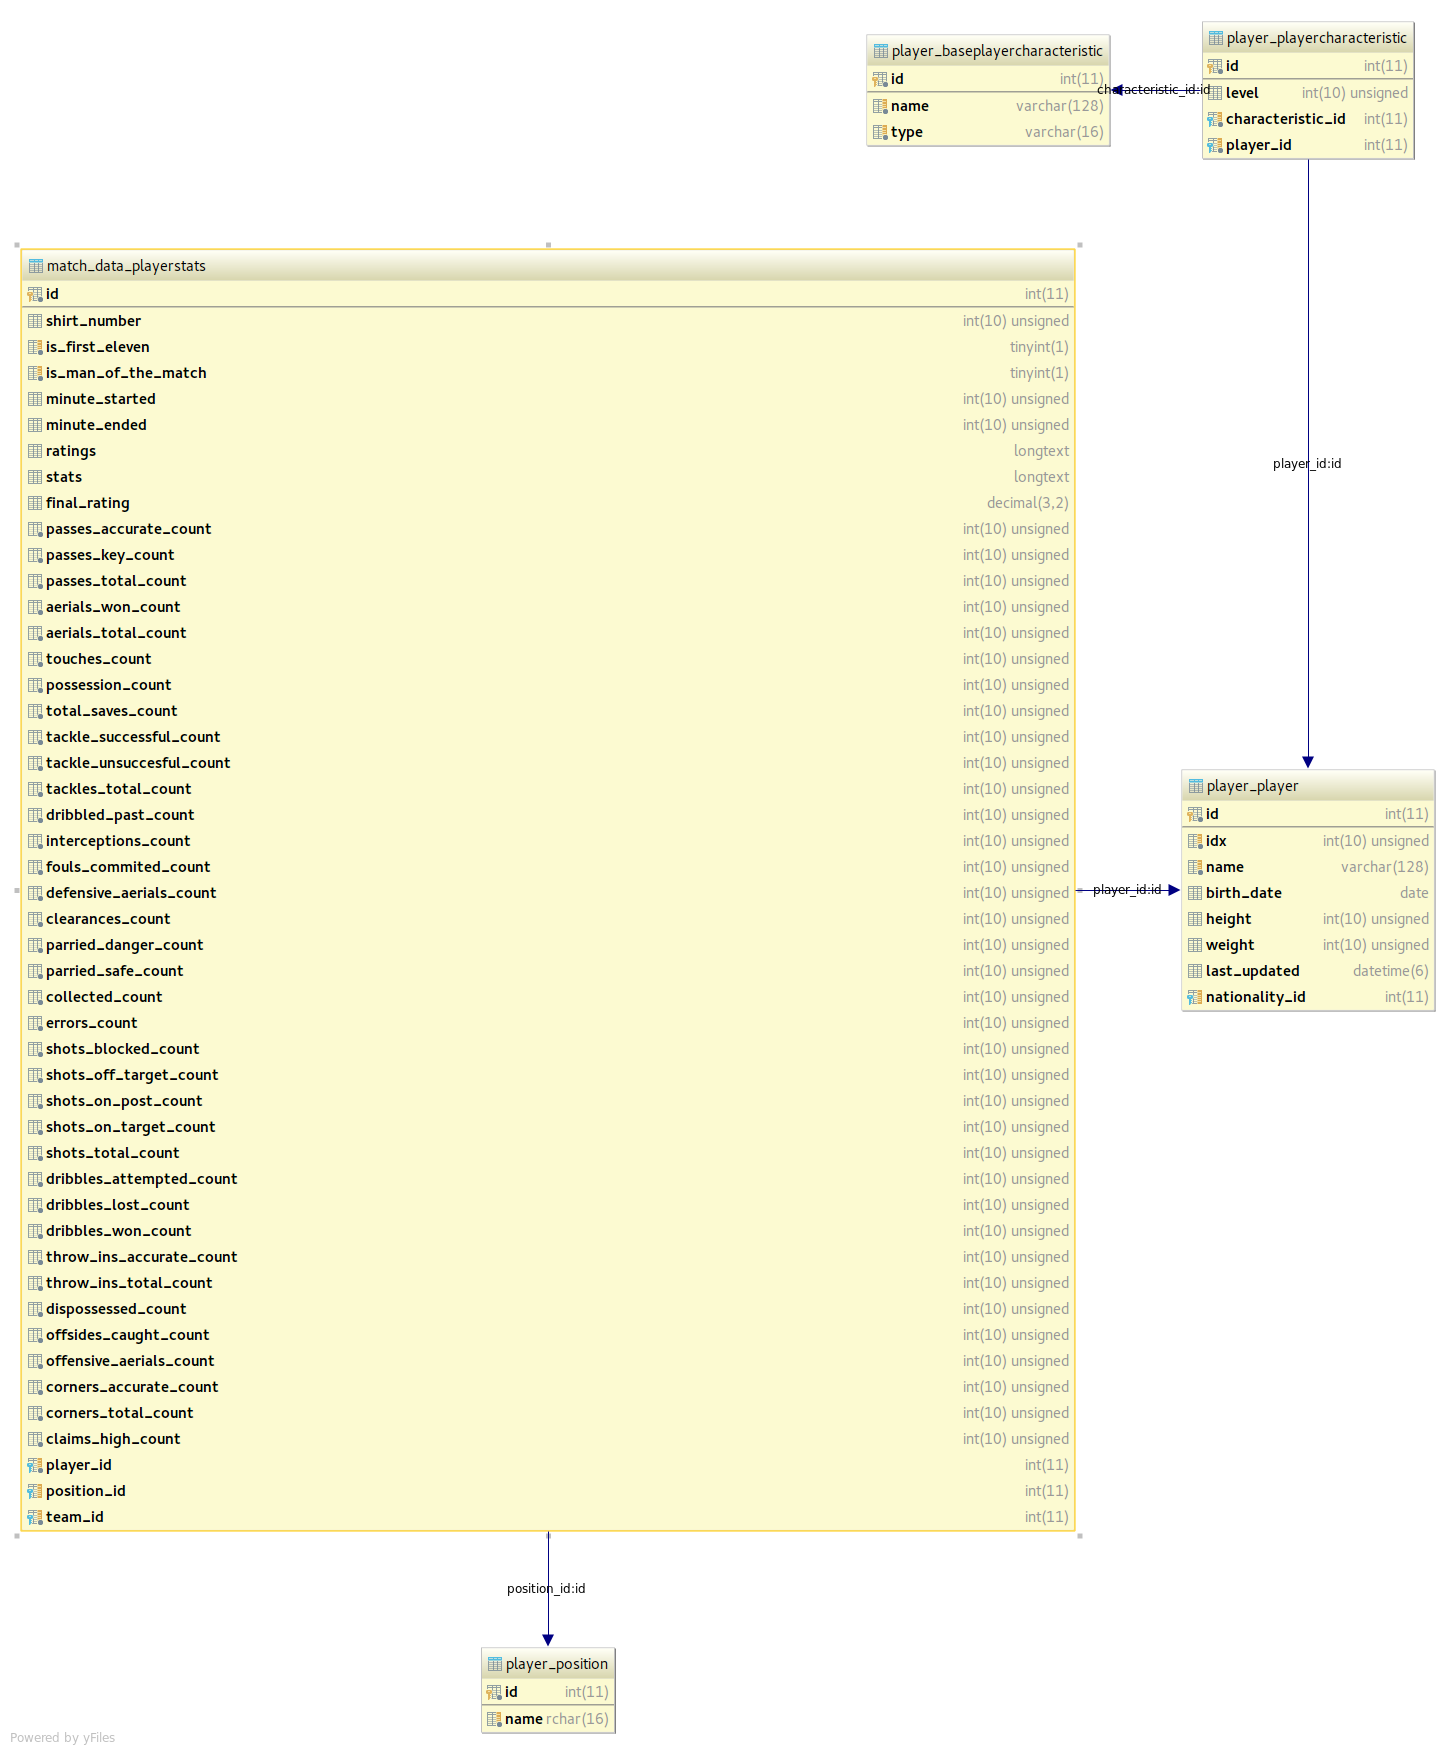
\includegraphics[width=0.9\textwidth]{database/player-stats.png}
    \caption{Database tables containing player related information.}
    \label{fig:database-player-stats}
\end{figure}


\subsection{Events}

\cref{fig:database-events} shows the database tables containing information concerning match events.

The \textit{event} table covers almost everything that takes place on the pitch during a match. An event is of a specific \textit{event type}, as listed in \cref{tab:whoscored-event-types}. An event takes place at specific \textit{position} on the pitch, at a given \textit{time} during the match. Most events are executed by a \textit{player} for one of the competing \textit{teams}. Some events, such as \textit{goals} and \textit{missed shots}, have related events. Events are marked with four Boolean attributes, \textit{is\_touch}, \textit{is\_goal}, \textit{is\_own\_goal}, \textit{is\_shot}. Events that span an area (such as shots, passes, etc.) are marked with an \textit{end position}. Events that enter the goal are marked with a \textit{goal position}, marking where it passed the goal mouth.

An event has a set of \textit{qualifiers}. Qualifiers describe the event in details. A qualifier is of a specific \textit{type}. \textit{Corner taken}, \textit{key pass}, \textit{angle}, \textit{length}, \textit{zone}, \textit{goal kick}, \textit{parried danger}, and \textit{hands} are some examples of qualifier types. Qualifiers such as \textit{angle}, \textit{length}, and \textit{zone} have associated \textit{values}. 

\begin{figure}
    \centering
    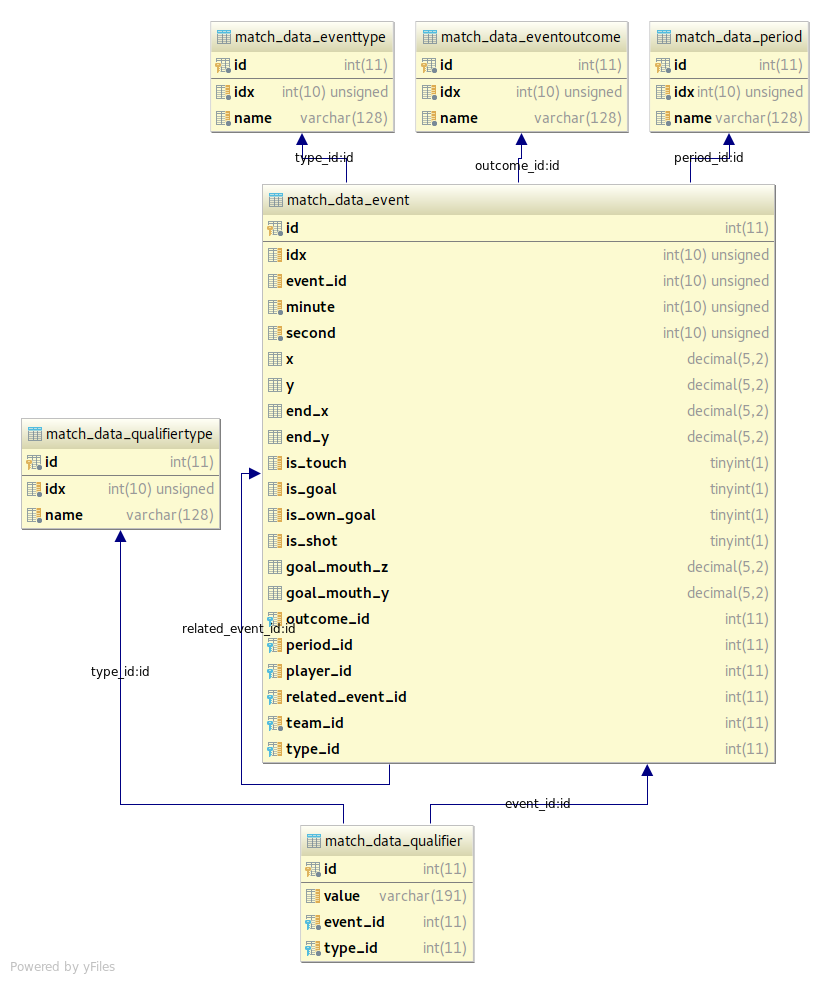
\includegraphics[width=0.9\textwidth]{database/event.png}
    \caption{Database tables containing event related information.}
    \label{fig:database-events}
\end{figure}


\subsection{Formations}

\cref{fig:database-formations} shows the database tables containing information concerning team formations.

\textit{Team formations} are included in matches with full level of details. A team formation concerns a specific \textit{team's} setup during a specific \textit{interval} of a match. Team formations have associated \textit{team captains}. A new team formation is created every time a team makes a substitution or rotates \textit{player positions}. A player position concerns a single player, and where on the pitch he plays at the given team formation.

Each team formation has an associated \textit{formation}. A formation signals how the players are arranged (4-4-2, 4-3-1, etc.).

\begin{figure}
    \centering
    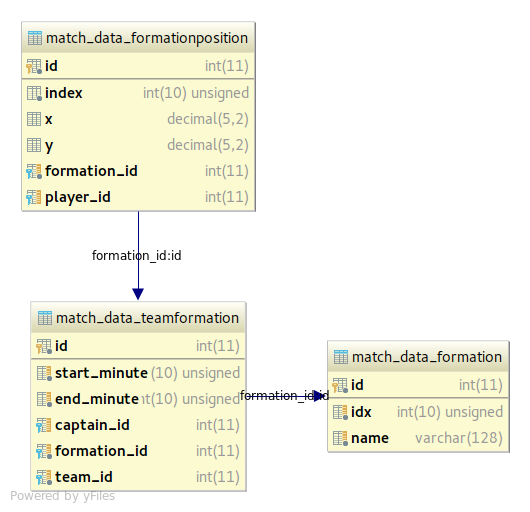
\includegraphics[width=0.9\textwidth]{database/formation.png}
    \caption{Database tables containing formation related information.}
    \label{fig:database-formations}
\end{figure}


\subsection{Substitutions}

\cref{fig:database-substitutions} shows the database tables containing information concerning substitutions.

Every time a player is substituted, a \textit{substitution} instance is created. A substitution contains information about what players were substituted at what time and period of the match.

\begin{figure}
    \centering
    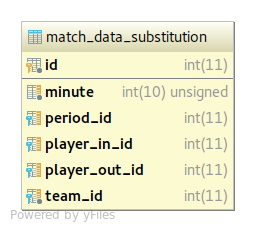
\includegraphics[width=0.5\textwidth]{database/substitution.png}
    \caption{Database table containing substitution related information.}
    \label{fig:database-substitutions}
\end{figure}